% Options for packages loaded elsewhere
\PassOptionsToPackage{unicode}{hyperref}
\PassOptionsToPackage{hyphens}{url}
\PassOptionsToPackage{dvipsnames,svgnames,x11names}{xcolor}
%
\documentclass[
  10pt,
]{scrartcl}

\usepackage{amsmath,amssymb}
\usepackage{setspace}
\usepackage{iftex}
\ifPDFTeX
  \usepackage[T1]{fontenc}
  \usepackage[utf8]{inputenc}
  \usepackage{textcomp} % provide euro and other symbols
\else % if luatex or xetex
  \usepackage{unicode-math}
  \defaultfontfeatures{Scale=MatchLowercase}
  \defaultfontfeatures[\rmfamily]{Ligatures=TeX,Scale=1}
\fi
\usepackage{lmodern}
\ifPDFTeX\else  
    % xetex/luatex font selection
    \setmainfont[]{Open Sans}
\fi
% Use upquote if available, for straight quotes in verbatim environments
\IfFileExists{upquote.sty}{\usepackage{upquote}}{}
\IfFileExists{microtype.sty}{% use microtype if available
  \usepackage[]{microtype}
  \UseMicrotypeSet[protrusion]{basicmath} % disable protrusion for tt fonts
}{}
\makeatletter
\@ifundefined{KOMAClassName}{% if non-KOMA class
  \IfFileExists{parskip.sty}{%
    \usepackage{parskip}
  }{% else
    \setlength{\parindent}{0pt}
    \setlength{\parskip}{6pt plus 2pt minus 1pt}}
}{% if KOMA class
  \KOMAoptions{parskip=half}}
\makeatother
\usepackage{xcolor}
\usepackage[vmargin=20mm,hmargin=20mm,headsep=5mm]{geometry}
\setlength{\emergencystretch}{3em} % prevent overfull lines
\setcounter{secnumdepth}{5}
% Make \paragraph and \subparagraph free-standing
\makeatletter
\ifx\paragraph\undefined\else
  \let\oldparagraph\paragraph
  \renewcommand{\paragraph}{
    \@ifstar
      \xxxParagraphStar
      \xxxParagraphNoStar
  }
  \newcommand{\xxxParagraphStar}[1]{\oldparagraph*{#1}\mbox{}}
  \newcommand{\xxxParagraphNoStar}[1]{\oldparagraph{#1}\mbox{}}
\fi
\ifx\subparagraph\undefined\else
  \let\oldsubparagraph\subparagraph
  \renewcommand{\subparagraph}{
    \@ifstar
      \xxxSubParagraphStar
      \xxxSubParagraphNoStar
  }
  \newcommand{\xxxSubParagraphStar}[1]{\oldsubparagraph*{#1}\mbox{}}
  \newcommand{\xxxSubParagraphNoStar}[1]{\oldsubparagraph{#1}\mbox{}}
\fi
\makeatother

\usepackage{color}
\usepackage{fancyvrb}
\newcommand{\VerbBar}{|}
\newcommand{\VERB}{\Verb[commandchars=\\\{\}]}
\DefineVerbatimEnvironment{Highlighting}{Verbatim}{commandchars=\\\{\}}
% Add ',fontsize=\small' for more characters per line
\usepackage{framed}
\definecolor{shadecolor}{RGB}{241,243,245}
\newenvironment{Shaded}{\begin{snugshade}}{\end{snugshade}}
\newcommand{\AlertTok}[1]{\textcolor[rgb]{0.68,0.00,0.00}{#1}}
\newcommand{\AnnotationTok}[1]{\textcolor[rgb]{0.37,0.37,0.37}{#1}}
\newcommand{\AttributeTok}[1]{\textcolor[rgb]{0.40,0.45,0.13}{#1}}
\newcommand{\BaseNTok}[1]{\textcolor[rgb]{0.68,0.00,0.00}{#1}}
\newcommand{\BuiltInTok}[1]{\textcolor[rgb]{0.00,0.23,0.31}{#1}}
\newcommand{\CharTok}[1]{\textcolor[rgb]{0.13,0.47,0.30}{#1}}
\newcommand{\CommentTok}[1]{\textcolor[rgb]{0.37,0.37,0.37}{#1}}
\newcommand{\CommentVarTok}[1]{\textcolor[rgb]{0.37,0.37,0.37}{\textit{#1}}}
\newcommand{\ConstantTok}[1]{\textcolor[rgb]{0.56,0.35,0.01}{#1}}
\newcommand{\ControlFlowTok}[1]{\textcolor[rgb]{0.00,0.23,0.31}{\textbf{#1}}}
\newcommand{\DataTypeTok}[1]{\textcolor[rgb]{0.68,0.00,0.00}{#1}}
\newcommand{\DecValTok}[1]{\textcolor[rgb]{0.68,0.00,0.00}{#1}}
\newcommand{\DocumentationTok}[1]{\textcolor[rgb]{0.37,0.37,0.37}{\textit{#1}}}
\newcommand{\ErrorTok}[1]{\textcolor[rgb]{0.68,0.00,0.00}{#1}}
\newcommand{\ExtensionTok}[1]{\textcolor[rgb]{0.00,0.23,0.31}{#1}}
\newcommand{\FloatTok}[1]{\textcolor[rgb]{0.68,0.00,0.00}{#1}}
\newcommand{\FunctionTok}[1]{\textcolor[rgb]{0.28,0.35,0.67}{#1}}
\newcommand{\ImportTok}[1]{\textcolor[rgb]{0.00,0.46,0.62}{#1}}
\newcommand{\InformationTok}[1]{\textcolor[rgb]{0.37,0.37,0.37}{#1}}
\newcommand{\KeywordTok}[1]{\textcolor[rgb]{0.00,0.23,0.31}{\textbf{#1}}}
\newcommand{\NormalTok}[1]{\textcolor[rgb]{0.00,0.23,0.31}{#1}}
\newcommand{\OperatorTok}[1]{\textcolor[rgb]{0.37,0.37,0.37}{#1}}
\newcommand{\OtherTok}[1]{\textcolor[rgb]{0.00,0.23,0.31}{#1}}
\newcommand{\PreprocessorTok}[1]{\textcolor[rgb]{0.68,0.00,0.00}{#1}}
\newcommand{\RegionMarkerTok}[1]{\textcolor[rgb]{0.00,0.23,0.31}{#1}}
\newcommand{\SpecialCharTok}[1]{\textcolor[rgb]{0.37,0.37,0.37}{#1}}
\newcommand{\SpecialStringTok}[1]{\textcolor[rgb]{0.13,0.47,0.30}{#1}}
\newcommand{\StringTok}[1]{\textcolor[rgb]{0.13,0.47,0.30}{#1}}
\newcommand{\VariableTok}[1]{\textcolor[rgb]{0.07,0.07,0.07}{#1}}
\newcommand{\VerbatimStringTok}[1]{\textcolor[rgb]{0.13,0.47,0.30}{#1}}
\newcommand{\WarningTok}[1]{\textcolor[rgb]{0.37,0.37,0.37}{\textit{#1}}}

\providecommand{\tightlist}{%
  \setlength{\itemsep}{0pt}\setlength{\parskip}{0pt}}\usepackage{longtable,booktabs,array}
\usepackage{calc} % for calculating minipage widths
% Correct order of tables after \paragraph or \subparagraph
\usepackage{etoolbox}
\makeatletter
\patchcmd\longtable{\par}{\if@noskipsec\mbox{}\fi\par}{}{}
\makeatother
% Allow footnotes in longtable head/foot
\IfFileExists{footnotehyper.sty}{\usepackage{footnotehyper}}{\usepackage{footnote}}
\makesavenoteenv{longtable}
\usepackage{graphicx}
\makeatletter
\def\maxwidth{\ifdim\Gin@nat@width>\linewidth\linewidth\else\Gin@nat@width\fi}
\def\maxheight{\ifdim\Gin@nat@height>\textheight\textheight\else\Gin@nat@height\fi}
\makeatother
% Scale images if necessary, so that they will not overflow the page
% margins by default, and it is still possible to overwrite the defaults
% using explicit options in \includegraphics[width, height, ...]{}
\setkeys{Gin}{width=\maxwidth,height=\maxheight,keepaspectratio}
% Set default figure placement to htbp
\makeatletter
\def\fps@figure{htbp}
\makeatother

\usepackage{booktabs}
\usepackage{longtable}
\usepackage{array}
\usepackage{multirow}
\usepackage{wrapfig}
\usepackage{float}
\usepackage{colortbl}
\usepackage{pdflscape}
\usepackage{tabu}
\usepackage{threeparttable}
\usepackage{threeparttablex}
\usepackage[normalem]{ulem}
\usepackage{makecell}
\usepackage{xcolor}
\usepackage{geometry}
\usepackage{tikz}
\usepackage{fontspec}
\usepackage{sectsty}
\usepackage{fancyhdr}
\usepackage{textpos}
\usepackage{orcidlink}
\definecolor{mypink}{RGB}{219, 48, 122}
\usepackage{graphics}
\usepackage{titlesec}
\usepackage{xcolor}

% Define custom color using RGB values
\definecolor{ssb-green}{rgb}{0.102, 0.616, 0.286}

% Set URL link color
\hypersetup{
  colorlinks=true,
  urlcolor=customlinkcolor % Use the custom color
}

% Load tocloft package and set dot leaders for all TOC entries
\usepackage{tocloft}
\renewcommand{\cftsecleader}{\cftdotfill{\cftdotsep}}
\renewcommand{\cftsubsecleader}{\cftdotfill{\cftdotsep}}
\renewcommand{\cftsubsubsecleader}{\cftdotfill{\cftdotsep}}

% Bold H1 headers and their page numbers in the TOC
\renewcommand{\cftsecfont}{\bfseries}
\renewcommand{\cftsecpagefont}{\bfseries}

% Load Roboto Condensed Bold font from system fonts
\newfontfamily\roboto{Roboto Condensed}[BoldFont={Roboto Condensed Bold}]

% Custom section fonts and sizes using titlesec
\titleformat{\section}
  {\roboto\bfseries\fontsize{18}{22}\selectfont}
  {\thesection}{1em}{}
\titleformat{\subsection}
  {\roboto\bfseries\fontsize{12}{22}\selectfont}
  {\thesubsection}{1em}{}
\titleformat{\subsubsection}
  {\roboto\bfseries\fontsize{11}{14}\selectfont}
  {\thesubsubsection}{1em}{}
\titleformat{\paragraph}
  {\roboto\bfseries\fontsize{11}{13}\selectfont}
  {\theparagraph}{1em}{}
\titleformat{\subparagraph}
  {\roboto\bfseries\fontsize{11}{13}\selectfont}
  {\thesubparagraph}{1em}{}

% Redefine numbering for sections and subsections
\renewcommand{\thesection}{\arabic{section}.}
\renewcommand{\thesubsection}{\arabic{section}.\arabic{subsection}}
\makeatletter
\@ifpackageloaded{tcolorbox}{}{\usepackage[skins,breakable]{tcolorbox}}
\@ifpackageloaded{fontawesome5}{}{\usepackage{fontawesome5}}
\definecolor{quarto-callout-color}{HTML}{909090}
\definecolor{quarto-callout-note-color}{HTML}{0758E5}
\definecolor{quarto-callout-important-color}{HTML}{CC1914}
\definecolor{quarto-callout-warning-color}{HTML}{EB9113}
\definecolor{quarto-callout-tip-color}{HTML}{00A047}
\definecolor{quarto-callout-caution-color}{HTML}{FC5300}
\definecolor{quarto-callout-color-frame}{HTML}{acacac}
\definecolor{quarto-callout-note-color-frame}{HTML}{4582ec}
\definecolor{quarto-callout-important-color-frame}{HTML}{d9534f}
\definecolor{quarto-callout-warning-color-frame}{HTML}{f0ad4e}
\definecolor{quarto-callout-tip-color-frame}{HTML}{02b875}
\definecolor{quarto-callout-caution-color-frame}{HTML}{fd7e14}
\makeatother
\makeatletter
\@ifpackageloaded{caption}{}{\usepackage{caption}}
\AtBeginDocument{%
\ifdefined\contentsname
  \renewcommand*\contentsname{Table of contents}
\else
  \newcommand\contentsname{Table of contents}
\fi
\ifdefined\listfigurename
  \renewcommand*\listfigurename{List of Figures}
\else
  \newcommand\listfigurename{List of Figures}
\fi
\ifdefined\listtablename
  \renewcommand*\listtablename{List of Tables}
\else
  \newcommand\listtablename{List of Tables}
\fi
\ifdefined\figurename
  \renewcommand*\figurename{Figure}
\else
  \newcommand\figurename{Figure}
\fi
\ifdefined\tablename
  \renewcommand*\tablename{Table}
\else
  \newcommand\tablename{Table}
\fi
}
\@ifpackageloaded{float}{}{\usepackage{float}}
\floatstyle{ruled}
\@ifundefined{c@chapter}{\newfloat{codelisting}{h}{lop}}{\newfloat{codelisting}{h}{lop}[chapter]}
\floatname{codelisting}{Listing}
\newcommand*\listoflistings{\listof{codelisting}{List of Listings}}
\makeatother
\makeatletter
\makeatother
\makeatletter
\@ifpackageloaded{caption}{}{\usepackage{caption}}
\@ifpackageloaded{subcaption}{}{\usepackage{subcaption}}
\makeatother

\ifLuaTeX
  \usepackage{selnolig}  % disable illegal ligatures
\fi
\usepackage[]{natbib}
\bibliographystyle{te}
\usepackage{bookmark}

\IfFileExists{xurl.sty}{\usepackage{xurl}}{} % add URL line breaks if available
\urlstyle{same} % disable monospaced font for URLs
\hypersetup{
  pdftitle={Tittel på SSB-rapport},
  pdfauthor={Forfatter1; Forfatter2},
  pdfkeywords={SSB, rapport, demo},
  colorlinks=true,
  linkcolor={blue},
  filecolor={Maroon},
  citecolor={ssb-green},
  urlcolor={ssb-green},
  pdfcreator={LaTeX via pandoc}}


\title{Tittel på SSB-rapport}
\usepackage{etoolbox}
\makeatletter
\providecommand{\subtitle}[1]{% add subtitle to \maketitle
  \apptocmd{\@title}{\par {\large #1 \par}}{}{}
}
\makeatother
\subtitle{Undertittel på SSB-rapport}
\author{Forfatter1 \and Forfatter2}
\date{}

\begin{document}
% Titlepage

% Definerer font som skal brukes i tittel og overskrifter (bold)   

    \begin{titlepage}
        \newgeometry{top=2cm, bottom=2cm, left=2cm, right=2cm} % Adjust margins as needed

        % Background image
        \begin{tikzpicture}[remember picture, overlay]
            \node[inner sep=0pt] at (current page.center) {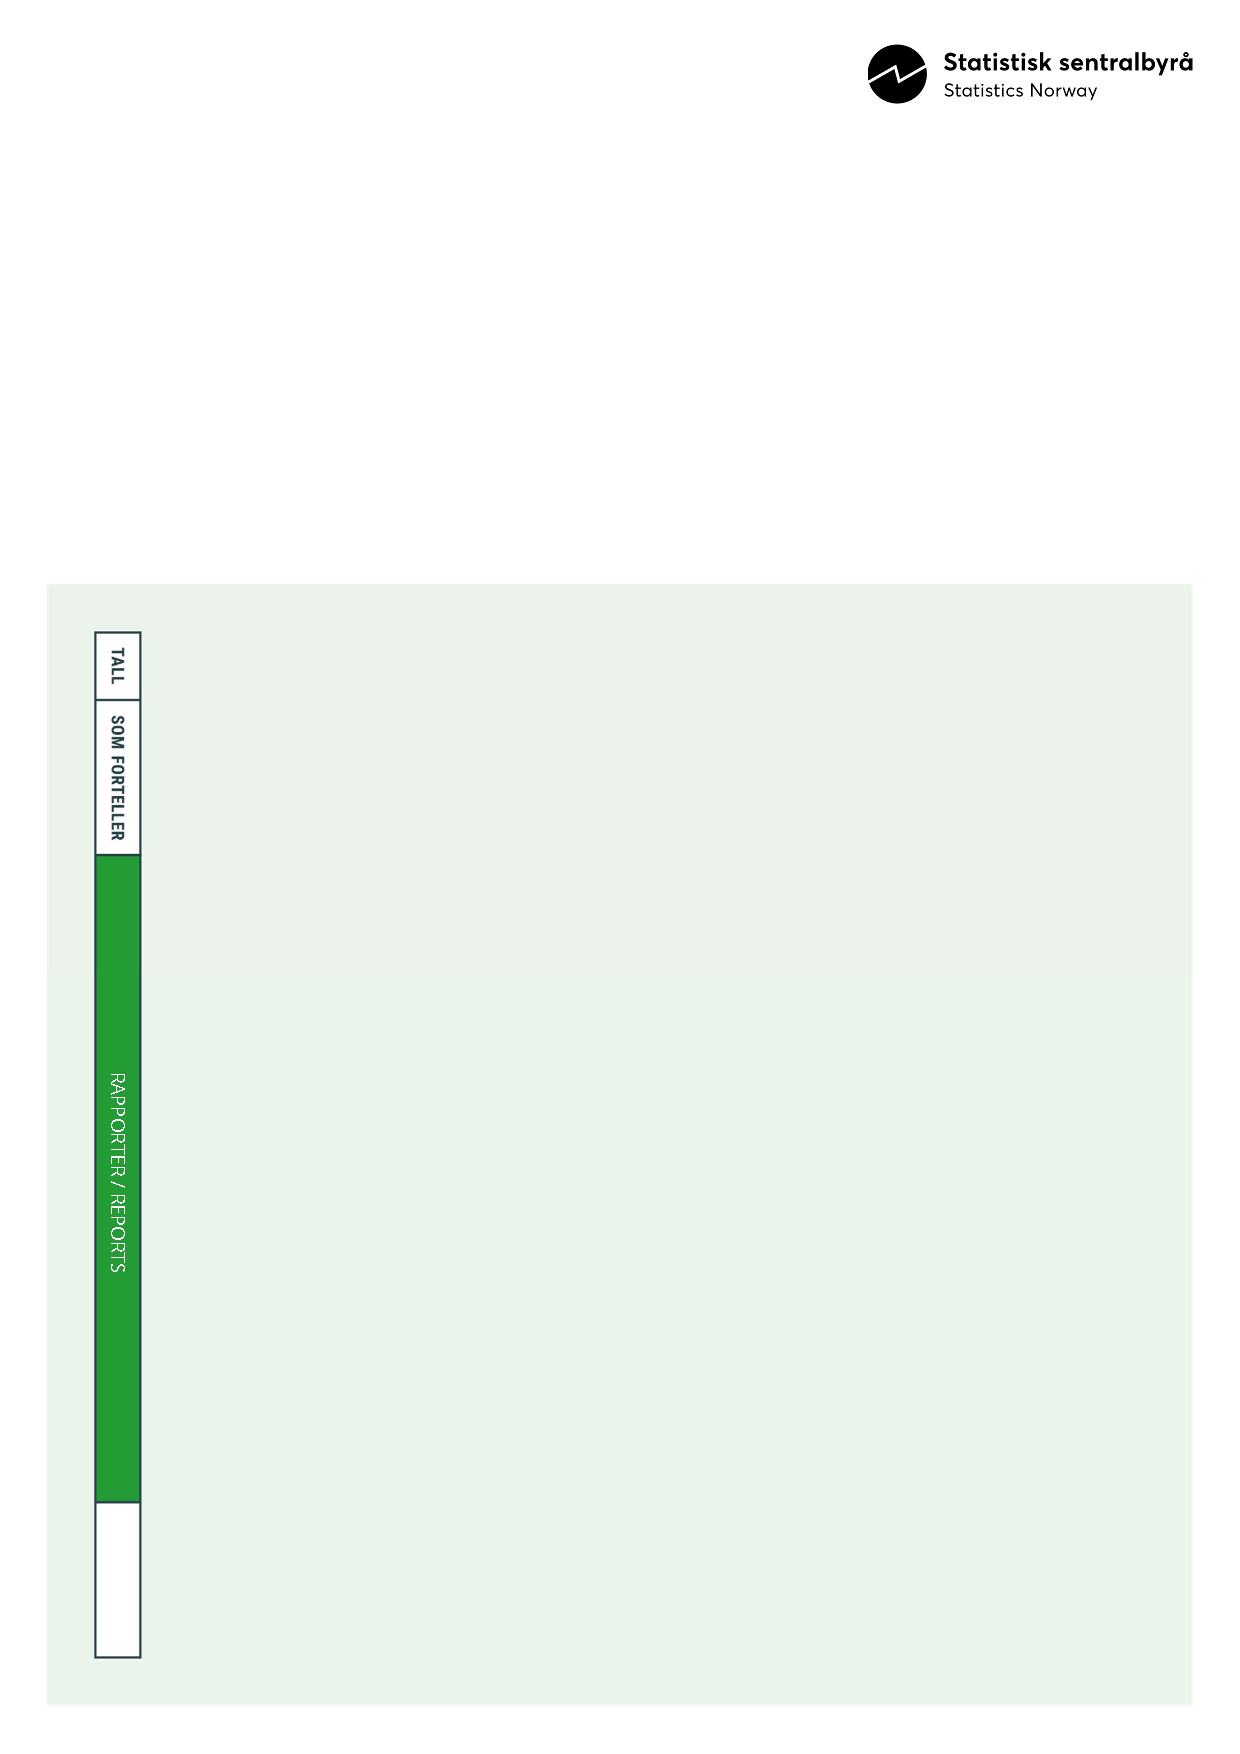
\includegraphics[width=\paperwidth,height=\paperheight]{frontpage.pdf}};
        \end{tikzpicture}

        % Foreground text
        \begin{tikzpicture}[remember picture, overlay]
            \node[align=center, text opacity=1, fill opacity=0] at (current page.center) {
                \begin{minipage}{\textwidth}
                    \vfill % Ensure vertical centering

                    % Title
                    \begin{flushleft}
                        \hspace*{-0.45cm} % Adjust this value to move the text to the right
                        \vspace*{-0cm} % Adjust this value to move the text upwards or downwards
                        {\roboto\textbf{\fontsize{40}{48}\selectfont Tittel
på SSB-rapport}}
                    \end{flushleft}

                    % Subtitle
                    \begin{flushleft}
                        \hspace*{-0.45cm} % Adjust this value to move the text to the right
                        \vspace*{5cm} % Adjust this value to move the text upwards or downwards
                        {\fontsize{14}{18}\selectfont Undertittel på
SSB-rapport}
                    \end{flushleft}

                    % Authors and Date
                    \begin{flushleft}
                        \hspace*{2cm} % Adjust this value to move the text to the right
                        \vspace*{11cm} % Adjust this value to move the text upwards or downwards
                        {\fontsize{10}{12}\selectfont \textsf{Forfatter1, Forfatter2}}
                        \vspace*{2cm} % Adjust this value to move the text upwards or downwards
                        {\Large \textsf{}}
                    \end{flushleft}

                    \vfill
                \end{minipage}
            };
        \end{tikzpicture}

        % Legger inn rapportnummer
                \begin{textblock}{3}(-0.1 ,12.5) % Adjust the coordinates (1.4, 14) to place the text within the page
            \rotatebox{270}{\fontsize{9}{11}\selectfont 2024/XX}
        \end{textblock}
        

    \end{titlepage}
    \restoregeometry

    
    
  
% Øyvind lager en kolofon-side
\newpage
\thispagestyle{empty}

I serien Rapporter publiseres analyser og kommenterte statistiske resultater fra ulike undersøkelser. Undersøkelser inkluderer både utvalgsundersøkelser, tellinger og registerbaserte undersøkelser.

\vskip 34em

\textcopyright
Statistisk sentralbyrå
\newline
Ved bruk av materiale fra denne publikasjonen skal Statistisk sentralbyrå oppgis som kilde.

\vskip 1em

Publisert: 1. desember 2024

\vskip 1em

ISBN 978-82-587-XXXX-X (trykt)
\newline
ISBN 978-82-587-YYYY-Y (elektronisk)
\newline
ISSN 0806-2056

\vskip 0.5em
\rule{\textwidth}{0.4pt}
\vskip 0.5em
\rule{\textwidth}{0.4pt}

\noindent
\textbf{Standardtegn i tabeller} \hfill \textbf{Symbol}
\newline
\rule{\textwidth}{0.4pt}

\noindent
\textbf{Ikke mulig oppgi tall} \hfill \textbf{.}
\newline
Tall finnes ikke på dette tidspunktet fordi kategorien ikke var i bruk da tallene ble samlet inn.
\newline
\rule{\textwidth}{0.4pt}

\noindent
\textbf{Tallgrunnlag mangler} \hfill \textbf{..}
\newline
Tall er ikke kommet inn i våre databaser eller er for usikre til å publiseres.
\newline
\rule{\textwidth}{0.4pt}

\noindent
\textbf{Vises ikke av konfidensialitetshensyn} \hfill \textbf{:}
\newline
Tall publiseres ikke for å unngå å identifisere personer eller virksomheter.
\newline
\rule{\textwidth}{0.4pt}

\noindent
\textbf{Desimalskilletegn} \hfill \textbf{,}
\newline
\rule{\textwidth}{0.4pt}

\clearpage


% Defines the header and footer used in the chapters
\fancypagestyle{ssb-report-footer-header}{
    \rhead{\fontsize{9}{11}\selectfont Tittel på SSB-rapport}
    \lhead{\fontsize{9}{11}\selectfont Rapporter 2024/XX}
    \fancyfoot[C]{\fontsize{9}{11}\selectfont \thepage} % Page number in the center
    \renewcommand{\headrulewidth}{0.0pt} % Thickness of the header line
    \renewcommand{\footrulewidth}{0.0pt} % Thickness of the footer line
}


% Apply the custom page style to the entire document
\pagestyle{ssb-report-footer-header}




% Øyvind lager Forord
\newpage
\section*{Forord}
\addcontentsline{toc}{section}{Forord}
Forordet skal være på maksimalt 250 ord og kan inneholde følgende
elementer:

Eventuell bakgrunn, informasjon om ev. tidligere versjoner, utgaver, og
hvor disse finnes, informasjon om ev. prosjektstøtte, oppdragsgiver
o.l., informasjon om ev. bidragsytere, ev. takksigelser, som bør
begrenses og ikke omfatte interne medarbeidere og oppdragsgivere.
\vskip 2em
Statistisk sentralbyrå, {Godkjenningsdato}
\vskip 1em
Navn på godkjenner
\clearpage

\newpage
\section*{Sammendrag}
\addcontentsline{toc}{section}{Sammendrag}
Sammendraget skal gi en kortfattet oversikt over innhold og resultater.
Det kan inneholde følgende elementer: Hovedformål med
rapporten/notatet/analysen, hovedkonklusjoner, ev. noe (veldig kort) om
metoder og modeller som er brukt.

Sammendraget skal ikke overstige én A4-side.
\newpage

\section*{Abstract}
\addcontentsline{toc}{section}{Abstract}
This is a summary of the report in english. Abstract er oversetting av
Sammendraget. Gjelder bare for serien Rapporter.

Abstract skal ikke overstige én A4-side
\newpage



\renewcommand*\contentsname{%
  {\roboto\bfseries\fontsize{18}{22}\selectfont Innhold} % Apply custom formatting
}
{
\hypersetup{linkcolor=}
\setcounter{tocdepth}{2}
\renewcommand{\contentsname}{%
  {\roboto\bfseries\fontsize{18}{22}\selectfont Innhold} % Apply custom formatting
}
\tableofcontents
\thispagestyle{ssb-report-footer-header} % Set custom page style for TOC
}

\newpage
\setstretch{1.5}
\section{Introduksjon}\label{sec-intro}

Denne teksten er et eksempel på hvordan teksten til en SSB-rapport
skrives med markdown og renderes med \href{https://quarto.org/}{Quarto}.
Quarto er et open source verktøy for publisiering av dokumenter som
kombinerer tekst og data-analyse. Det gir muligheten til å lage
dynamiske rapporter, presentasjoner, nettsider og bøker med integrert
kode.

\subsection{Kom i gang}\label{kom-i-gang}

For å bruke denne templaten kan du klone repoet og begynne å redigere på
\texttt{template.qmd}.

\begin{Shaded}
\begin{Highlighting}[]
\FunctionTok{git}\NormalTok{ clone https://github.com/statisticsnorway/ssb{-}quarto{-}report.git}
\end{Highlighting}
\end{Shaded}

Deretter kan du kan gå inn i mappen \texttt{cd\ ssb-quarto-report} og
rendere eksempelfilen:

\begin{Shaded}
\begin{Highlighting}[]
\ExtensionTok{quarto}\NormalTok{ preview ssb/template.qmd}
\end{Highlighting}
\end{Shaded}

Det gir deg en forhåndsvisning av dokumentet som oppdateres fortløpende
når du gjør endringer i \texttt{template.qmd}-filen.

\subsubsection{Metadata}\label{metadata}

De første endringene man gjør i \texttt{template.qmd} er typisk å endre
metadataene som ligger i toppen av fila. Der oppgir du tittel,
undertittel, forfattere, forord, godkjenningsdato, etc.. Verdiene som
oppgis her vil bli lagt inn i den ferdig renderte pdf-en på de riktige
stedene i dokumentet. Metadataene kan derfor se slik ut:

\begin{Shaded}
\begin{Highlighting}[]
\FunctionTok{title}\KeywordTok{:}\AttributeTok{ }\StringTok{"Kvantitative svar på kompliserte spørsmål"}
\FunctionTok{subtitle}\KeywordTok{:}\AttributeTok{ }\StringTok{"En spennende rapport fra SSB"}
\FunctionTok{approved{-}date}\KeywordTok{:}\AttributeTok{ 1. januar 2025}
\FunctionTok{approved{-}by}\KeywordTok{:}\AttributeTok{ Daniel Direktør}
\FunctionTok{rapportnr}\KeywordTok{:}\AttributeTok{ }\StringTok{"2025/11"}
\FunctionTok{publisert{-}dato}\KeywordTok{:}\AttributeTok{ 1. desember 2024}
\FunctionTok{isbn{-}t}\KeywordTok{:}\AttributeTok{ 9999{-}9}
\FunctionTok{isbn{-}e}\KeywordTok{:}\AttributeTok{ 8888{-}8}
\FunctionTok{format}\KeywordTok{:}
\AttributeTok{  }\FunctionTok{ssb{-}pdf}\KeywordTok{:}
\AttributeTok{    }\FunctionTok{keep{-}tex}\KeywordTok{:}\AttributeTok{ }\CharTok{true}\AttributeTok{  }
\AttributeTok{  }\FunctionTok{ssb{-}html}\KeywordTok{:}\AttributeTok{ default}
\FunctionTok{author}\KeywordTok{:}
\AttributeTok{  }\KeywordTok{{-}}\AttributeTok{ }\FunctionTok{name}\KeywordTok{:}\AttributeTok{ Ståle Statistiker}
\end{Highlighting}
\end{Shaded}

Hvis du gjør endringene over og trykker save så ser du at disse verdiene
blir satt i forhåndsvisningen av pdf-en. Når du er fornøyd så kan du
rendere den endelige versjonen ved å kjøre følende i terminalen:

\begin{Shaded}
\begin{Highlighting}[]
\ExtensionTok{quarto}\NormalTok{ render template.qmd}
\end{Highlighting}
\end{Shaded}

\subsubsection{Skrive artikkel}\label{skrive-artikkel}

Å skrive selve artikkelen kan man gjøre ved å skrive markdown i
\texttt{template.qmd}. Markdown-syntaxen er godt dokumentert i
\href{https://quarto.org/docs/authoring/markdown-basics.html}{Quart-manualen}.
Det er også greit å vite at Quarto bruker
\href{https://pandoc.org/}{Pandoc} under panseret.

Måten dokumentet pdf-rapporten blir til på er at:

\begin{enumerate}
\def\labelenumi{\arabic{enumi}.}
\tightlist
\item
  All informasjon\footnote{Metadata og markdown} blir konvertert til
  formatet \href{https://pandoc.org/lua-filters.html}{Pandoc AST}
\item
  For generering av PDF blir Pandoc AST først konvertert til Latex, og
  deretter PDF.
\item
  For generering av docx-filer blir Pandoc AST konvertert direkte til
  docx.
\item
  For generering av html blir Pandoc AST konvertert direkte til html.
\end{enumerate}

For de som ønsker å tilpasse templaten til sine behov, så må man derfor
forholde seg til mellomformatet Pandoc AST, og hvis man ønsker at
sluttproduktet skal være en pdf, så må man også ha basis kunnskap om
Latex. Hvis man ønsker å gjøre endringer på Pandoc AST formatet direkte
som en del av renderingen, så kan man skrive såkalte \textbf{filtre}
eller \textbf{shortcodes} i Lua som prosesserer Pandoc AST direkte ved
rendering. Men dette er kun nødvendig for avanserte brukere som ønsker å
gjøre utvikling på templaten.

Av metadatene over ser vi at man kan velge å beholde den Latex-koden som
generer pdf-fila, \texttt{keep-tex:\ true}. Det kan være nyttig for de
som lurer på hvordan konvertering fra markdown, via AST, har blitt
tolket som Latex. Man kan også bruke den til å manipulere Latex-koden
direkte og deretter rendere.

\subsubsection{Hvem passer dette for?}\label{hvem-passer-dette-for}

Denne arbeidsflyten kan passe for de i SSB som skriver rapporter der
data er en viktig del av innholdet. Siden denne måten å skrive på
tillater forfatteren å skrive der man har tilgang til data, samtidig som
man kan blande tekst, kode og output på en enkel måte. En stor fordel
med dette er at rapporten kan genereres på samme måte som statistikk
genereres, ved å kjøre tekstfiler. På den måten kan man versjonhåndtere
dokumentet på GitHub, kjøre dokumentet på nytt hvis dataene endrer seg,
og dokumentere tall og figurere som en del av skrivingen.

\section{Komponenter}\label{komponenter}

Når man skriver dokumenter skal man følge den visuelle profilen til SSB.
Defor må tabeller, figurer, forklaringsbokser, og kildehenvisninger
følge SSBs profil.

\subsection{Tabeller}\label{tabeller}

Å lage tabeller kan gjøres på mange forskjellige måter i et
Quarto-dokument. Man kan lage tabeller ved å bruke R- og
Python-biblioteker som produserer markdown, Latex eller bilder. Man kan
også legge inn ren Latex i denne filen.

\subsubsection{Markdown}\label{markdown}

Man kan lage en tabell i Excel og
\href{https://tabletomarkdown.com/convert-spreadsheet-to-markdown/}{transformere
den til markdown}, som Quarto kan rendere til pdf eller html. Man kan
også bruke R- og Python-pakker som genererer markdown-tabeller. Denne
koden genererer en enkel tabell:

\begin{Shaded}
\begin{Highlighting}[]
\InformationTok{\textasciigrave{}\textasciigrave{}\textasciigrave{}\{r\}}
\InformationTok{\#| echo: false}

\InformationTok{library(knitr)}

\InformationTok{\# Create a simple data frame}
\InformationTok{df \textless{}{-} data.frame(}
\InformationTok{  Name = c("John", "Jane", "Doe"),}
\InformationTok{  Age = c(23, 35, 45),}
\InformationTok{  Occupation = c("Engineer", "Doctor", "Artist")}
\InformationTok{)}

\InformationTok{\# Convert the data frame to a markdown table}
\InformationTok{markdown\_table \textless{}{-} knitr::kable(df, format = "markdown")}

\InformationTok{\# Print the markdown table}
\InformationTok{markdown\_table}
\InformationTok{\textasciigrave{}\textasciigrave{}\textasciigrave{}}
\end{Highlighting}
\end{Shaded}

\begin{longtable}[]{@{}lrl@{}}

\caption{\label{tbl-md}En enkel tabell med markdown}

\tabularnewline

\toprule\noalign{}
Name & Age & Occupation \\
\midrule\noalign{}
\endhead
\bottomrule\noalign{}
\endlastfoot
John & 23 & Engineer \\
Jane & 35 & Doctor \\
Doe & 45 & Artist \\

\end{longtable}

Vi kunne også laget en tabell uten pakker. Denne teksten genererer også
en enkel makrdown-tabell:

\begin{Shaded}
\begin{Highlighting}[]
\InformationTok{\textasciigrave{}\textasciigrave{}\textasciigrave{}\{markdown\}}
\InformationTok{| Default | Left | Right | Center |}
\InformationTok{|{-}{-}{-}{-}{-}{-}{-}{-}:|{-}{-}{-}{-}{-}:|{-}{-}{-}{-}{-}{-}:|:{-}{-}{-}{-}{-}{-}:|}
\InformationTok{| 12      | 12   |    12 |   12   |}
\InformationTok{| 123     | 123  |   123 |  123   |}
\InformationTok{| 1       | 1    |     1 |   1    |}
\InformationTok{: Et annet eksempel med rå markdown \{\#tbl{-}md1 tbl{-}colwidths="[25,25]"\}}
\InformationTok{\textasciigrave{}\textasciigrave{}\textasciigrave{}}
\end{Highlighting}
\end{Shaded}

\begin{longtable}[]{@{}
  >{\raggedleft\arraybackslash}p{(\columnwidth - 6\tabcolsep) * \real{0.2500}}
  >{\raggedleft\arraybackslash}p{(\columnwidth - 6\tabcolsep) * \real{0.2500}}
  >{\raggedleft\arraybackslash}p{(\columnwidth - 6\tabcolsep) * \real{0.2500}}
  >{\centering\arraybackslash}p{(\columnwidth - 6\tabcolsep) * \real{0.2500}}@{}}
\caption{Et annet eksempel med rå
markdown}\label{tbl-md1}\tabularnewline
\toprule\noalign{}
\begin{minipage}[b]{\linewidth}\raggedleft
Default
\end{minipage} & \begin{minipage}[b]{\linewidth}\raggedleft
Left
\end{minipage} & \begin{minipage}[b]{\linewidth}\raggedleft
Right
\end{minipage} & \begin{minipage}[b]{\linewidth}\centering
Center
\end{minipage} \\
\midrule\noalign{}
\endfirsthead
\toprule\noalign{}
\begin{minipage}[b]{\linewidth}\raggedleft
Default
\end{minipage} & \begin{minipage}[b]{\linewidth}\raggedleft
Left
\end{minipage} & \begin{minipage}[b]{\linewidth}\raggedleft
Right
\end{minipage} & \begin{minipage}[b]{\linewidth}\centering
Center
\end{minipage} \\
\midrule\noalign{}
\endhead
\bottomrule\noalign{}
\endlastfoot
12 & 12 & 12 & 12 \\
123 & 123 & 123 & 123 \\
1 & 1 & 1 & 1 \\
\end{longtable}

Vi kan referere til tabellene ved å bruke Table~\ref{tbl-md},
Table~\ref{tbl-md1}. De blir også automatisk nummerert og listet ut i
Tabellregisteret på slutten av dokumentet.

\subsubsection{Latex}\label{latex}

Man kan også bruke Latex til å generere tabeller, enten vha rå Latex
eller R- eller Python-pakker. Her er et eksempel på hvordan man kan
bruke R-pakken
\href{https://haozhu233.github.io/kableExtra/awesome_table_in_pdf.pdf}{kableExtra}
for enkelt lage avanserte Latex-tabeller:

\begin{Shaded}
\begin{Highlighting}[]
\FunctionTok{library}\NormalTok{(kableExtra)}
\NormalTok{dt }\OtherTok{\textless{}{-}}\NormalTok{ mtcars[}\DecValTok{1}\SpecialCharTok{:}\DecValTok{5}\NormalTok{, }\DecValTok{1}\SpecialCharTok{:}\DecValTok{6}\NormalTok{]}
\FunctionTok{kbl}\NormalTok{(dt)}
\NormalTok{long\_dt }\OtherTok{\textless{}{-}} \FunctionTok{rbind}\NormalTok{(mtcars, mtcars)}
\FunctionTok{kbl}\NormalTok{(long\_dt, }\AttributeTok{longtable =}\NormalTok{ T, }\AttributeTok{booktabs =}\NormalTok{ T) }\SpecialCharTok{\%\textgreater{}\%}
  \FunctionTok{add\_header\_above}\NormalTok{(}\FunctionTok{c}\NormalTok{(}\StringTok{" "}\NormalTok{, }\StringTok{"Group 1"} \OtherTok{=} \DecValTok{5}\NormalTok{, }\StringTok{"Group 2"} \OtherTok{=} \DecValTok{6}\NormalTok{)) }\SpecialCharTok{\%\textgreater{}\%}
  \FunctionTok{kable\_styling}\NormalTok{(}\AttributeTok{latex\_options =} \FunctionTok{c}\NormalTok{(}\StringTok{"repeat\_header"}\NormalTok{, }\StringTok{"striped"}\NormalTok{)) }\SpecialCharTok{\%\textgreater{}\%}
  \FunctionTok{footnote}\NormalTok{(}\AttributeTok{general =} \StringTok{"Here is a general comments of the table. "}\NormalTok{,}
          \AttributeTok{number =} \FunctionTok{c}\NormalTok{(}\StringTok{"Footnote 1; "}\NormalTok{, }\StringTok{"Footnote 2; "}\NormalTok{),}
          \AttributeTok{alphabet =} \FunctionTok{c}\NormalTok{(}\StringTok{"Footnote A; "}\NormalTok{, }\StringTok{"Footnote B; "}\NormalTok{),}
          \AttributeTok{symbol =} \FunctionTok{c}\NormalTok{(}\StringTok{"Footnote Symbol 1; "}\NormalTok{, }\StringTok{"Footnote Symbol 2"}\NormalTok{)}
\NormalTok{          )}
\end{Highlighting}
\end{Shaded}

\begin{tabular}[t]{l|r|r|r|r|r|r}
\hline
  & mpg & cyl & disp & hp & drat & wt\\
\hline
Mazda RX4 & 21.0 & 6 & 160 & 110 & 3.90 & 2.620\\
\hline
Mazda RX4 Wag & 21.0 & 6 & 160 & 110 & 3.90 & 2.875\\
\hline
Datsun 710 & 22.8 & 4 & 108 & 93 & 3.85 & 2.320\\
\hline
Hornet 4 Drive & 21.4 & 6 & 258 & 110 & 3.08 & 3.215\\
\hline
Hornet Sportabout & 18.7 & 8 & 360 & 175 & 3.15 & 3.440\\
\hline
\end{tabular}

\begin{longtable}[t]{lrrrrrrrrrrr}

\caption{\label{tbl-latex}En avansert tabell med Latex/booktabs}

\tabularnewline

\toprule
\multicolumn{1}{c}{ } & \multicolumn{5}{c}{Group 1} & \multicolumn{6}{c}{Group 2} \\
\cmidrule(l{3pt}r{3pt}){2-6} \cmidrule(l{3pt}r{3pt}){7-12}
  & mpg & cyl & disp & hp & drat & wt & qsec & vs & am & gear & carb\\
\midrule
\endfirsthead
\multicolumn{12}{@{}l}{\textit{(continued)}}\\
\toprule
\multicolumn{1}{c}{ } & \multicolumn{5}{c}{Group 1} & \multicolumn{6}{c}{Group 2} \\
\cmidrule(l{3pt}r{3pt}){2-6} \cmidrule(l{3pt}r{3pt}){7-12}
  & mpg & cyl & disp & hp & drat & wt & qsec & vs & am & gear & carb\\
\midrule
\endhead

\endfoot
\bottomrule
\multicolumn{12}{l}{\rule{0pt}{1em}\textit{Note: }}\\
\multicolumn{12}{l}{\rule{0pt}{1em}Here is a general comments of the table. }\\
\multicolumn{12}{l}{\rule{0pt}{1em}\textsuperscript{1} Footnote 1; }\\
\multicolumn{12}{l}{\rule{0pt}{1em}\textsuperscript{2} Footnote 2; }\\
\multicolumn{12}{l}{\rule{0pt}{1em}\textsuperscript{a} Footnote A; }\\
\multicolumn{12}{l}{\rule{0pt}{1em}\textsuperscript{b} Footnote B; }\\
\multicolumn{12}{l}{\rule{0pt}{1em}\textsuperscript{*} Footnote Symbol 1; }\\
\multicolumn{12}{l}{\rule{0pt}{1em}\textsuperscript{\dag} Footnote Symbol 2}\\
\endlastfoot
\cellcolor{gray!10}{Mazda RX4} & \cellcolor{gray!10}{21.0} & \cellcolor{gray!10}{6} & \cellcolor{gray!10}{160.0} & \cellcolor{gray!10}{110} & \cellcolor{gray!10}{3.90} & \cellcolor{gray!10}{2.620} & \cellcolor{gray!10}{16.46} & \cellcolor{gray!10}{0} & \cellcolor{gray!10}{1} & \cellcolor{gray!10}{4} & \cellcolor{gray!10}{4}\\
Mazda RX4 Wag & 21.0 & 6 & 160.0 & 110 & 3.90 & 2.875 & 17.02 & 0 & 1 & 4 & 4\\
\cellcolor{gray!10}{Datsun 710} & \cellcolor{gray!10}{22.8} & \cellcolor{gray!10}{4} & \cellcolor{gray!10}{108.0} & \cellcolor{gray!10}{93} & \cellcolor{gray!10}{3.85} & \cellcolor{gray!10}{2.320} & \cellcolor{gray!10}{18.61} & \cellcolor{gray!10}{1} & \cellcolor{gray!10}{1} & \cellcolor{gray!10}{4} & \cellcolor{gray!10}{1}\\
Hornet 4 Drive & 21.4 & 6 & 258.0 & 110 & 3.08 & 3.215 & 19.44 & 1 & 0 & 3 & 1\\
\cellcolor{gray!10}{Hornet Sportabout} & \cellcolor{gray!10}{18.7} & \cellcolor{gray!10}{8} & \cellcolor{gray!10}{360.0} & \cellcolor{gray!10}{175} & \cellcolor{gray!10}{3.15} & \cellcolor{gray!10}{3.440} & \cellcolor{gray!10}{17.02} & \cellcolor{gray!10}{0} & \cellcolor{gray!10}{0} & \cellcolor{gray!10}{3} & \cellcolor{gray!10}{2}\\
\addlinespace
Valiant & 18.1 & 6 & 225.0 & 105 & 2.76 & 3.460 & 20.22 & 1 & 0 & 3 & 1\\
\cellcolor{gray!10}{Duster 360} & \cellcolor{gray!10}{14.3} & \cellcolor{gray!10}{8} & \cellcolor{gray!10}{360.0} & \cellcolor{gray!10}{245} & \cellcolor{gray!10}{3.21} & \cellcolor{gray!10}{3.570} & \cellcolor{gray!10}{15.84} & \cellcolor{gray!10}{0} & \cellcolor{gray!10}{0} & \cellcolor{gray!10}{3} & \cellcolor{gray!10}{4}\\
Merc 240D & 24.4 & 4 & 146.7 & 62 & 3.69 & 3.190 & 20.00 & 1 & 0 & 4 & 2\\
\cellcolor{gray!10}{Merc 230} & \cellcolor{gray!10}{22.8} & \cellcolor{gray!10}{4} & \cellcolor{gray!10}{140.8} & \cellcolor{gray!10}{95} & \cellcolor{gray!10}{3.92} & \cellcolor{gray!10}{3.150} & \cellcolor{gray!10}{22.90} & \cellcolor{gray!10}{1} & \cellcolor{gray!10}{0} & \cellcolor{gray!10}{4} & \cellcolor{gray!10}{2}\\
Merc 280 & 19.2 & 6 & 167.6 & 123 & 3.92 & 3.440 & 18.30 & 1 & 0 & 4 & 4\\
\addlinespace
\cellcolor{gray!10}{Merc 280C} & \cellcolor{gray!10}{17.8} & \cellcolor{gray!10}{6} & \cellcolor{gray!10}{167.6} & \cellcolor{gray!10}{123} & \cellcolor{gray!10}{3.92} & \cellcolor{gray!10}{3.440} & \cellcolor{gray!10}{18.90} & \cellcolor{gray!10}{1} & \cellcolor{gray!10}{0} & \cellcolor{gray!10}{4} & \cellcolor{gray!10}{4}\\
Merc 450SE & 16.4 & 8 & 275.8 & 180 & 3.07 & 4.070 & 17.40 & 0 & 0 & 3 & 3\\
\cellcolor{gray!10}{Merc 450SL} & \cellcolor{gray!10}{17.3} & \cellcolor{gray!10}{8} & \cellcolor{gray!10}{275.8} & \cellcolor{gray!10}{180} & \cellcolor{gray!10}{3.07} & \cellcolor{gray!10}{3.730} & \cellcolor{gray!10}{17.60} & \cellcolor{gray!10}{0} & \cellcolor{gray!10}{0} & \cellcolor{gray!10}{3} & \cellcolor{gray!10}{3}\\
Merc 450SLC & 15.2 & 8 & 275.8 & 180 & 3.07 & 3.780 & 18.00 & 0 & 0 & 3 & 3\\
\cellcolor{gray!10}{Cadillac Fleetwood} & \cellcolor{gray!10}{10.4} & \cellcolor{gray!10}{8} & \cellcolor{gray!10}{472.0} & \cellcolor{gray!10}{205} & \cellcolor{gray!10}{2.93} & \cellcolor{gray!10}{5.250} & \cellcolor{gray!10}{17.98} & \cellcolor{gray!10}{0} & \cellcolor{gray!10}{0} & \cellcolor{gray!10}{3} & \cellcolor{gray!10}{4}\\
\addlinespace
Lincoln Continental & 10.4 & 8 & 460.0 & 215 & 3.00 & 5.424 & 17.82 & 0 & 0 & 3 & 4\\
\cellcolor{gray!10}{Chrysler Imperial} & \cellcolor{gray!10}{14.7} & \cellcolor{gray!10}{8} & \cellcolor{gray!10}{440.0} & \cellcolor{gray!10}{230} & \cellcolor{gray!10}{3.23} & \cellcolor{gray!10}{5.345} & \cellcolor{gray!10}{17.42} & \cellcolor{gray!10}{0} & \cellcolor{gray!10}{0} & \cellcolor{gray!10}{3} & \cellcolor{gray!10}{4}\\
Fiat 128 & 32.4 & 4 & 78.7 & 66 & 4.08 & 2.200 & 19.47 & 1 & 1 & 4 & 1\\
\cellcolor{gray!10}{Honda Civic} & \cellcolor{gray!10}{30.4} & \cellcolor{gray!10}{4} & \cellcolor{gray!10}{75.7} & \cellcolor{gray!10}{52} & \cellcolor{gray!10}{4.93} & \cellcolor{gray!10}{1.615} & \cellcolor{gray!10}{18.52} & \cellcolor{gray!10}{1} & \cellcolor{gray!10}{1} & \cellcolor{gray!10}{4} & \cellcolor{gray!10}{2}\\
Toyota Corolla & 33.9 & 4 & 71.1 & 65 & 4.22 & 1.835 & 19.90 & 1 & 1 & 4 & 1\\
\addlinespace
\cellcolor{gray!10}{Toyota Corona} & \cellcolor{gray!10}{21.5} & \cellcolor{gray!10}{4} & \cellcolor{gray!10}{120.1} & \cellcolor{gray!10}{97} & \cellcolor{gray!10}{3.70} & \cellcolor{gray!10}{2.465} & \cellcolor{gray!10}{20.01} & \cellcolor{gray!10}{1} & \cellcolor{gray!10}{0} & \cellcolor{gray!10}{3} & \cellcolor{gray!10}{1}\\
Dodge Challenger & 15.5 & 8 & 318.0 & 150 & 2.76 & 3.520 & 16.87 & 0 & 0 & 3 & 2\\
\cellcolor{gray!10}{AMC Javelin} & \cellcolor{gray!10}{15.2} & \cellcolor{gray!10}{8} & \cellcolor{gray!10}{304.0} & \cellcolor{gray!10}{150} & \cellcolor{gray!10}{3.15} & \cellcolor{gray!10}{3.435} & \cellcolor{gray!10}{17.30} & \cellcolor{gray!10}{0} & \cellcolor{gray!10}{0} & \cellcolor{gray!10}{3} & \cellcolor{gray!10}{2}\\
Camaro Z28 & 13.3 & 8 & 350.0 & 245 & 3.73 & 3.840 & 15.41 & 0 & 0 & 3 & 4\\
\cellcolor{gray!10}{Pontiac Firebird} & \cellcolor{gray!10}{19.2} & \cellcolor{gray!10}{8} & \cellcolor{gray!10}{400.0} & \cellcolor{gray!10}{175} & \cellcolor{gray!10}{3.08} & \cellcolor{gray!10}{3.845} & \cellcolor{gray!10}{17.05} & \cellcolor{gray!10}{0} & \cellcolor{gray!10}{0} & \cellcolor{gray!10}{3} & \cellcolor{gray!10}{2}\\
\addlinespace
Fiat X1-9 & 27.3 & 4 & 79.0 & 66 & 4.08 & 1.935 & 18.90 & 1 & 1 & 4 & 1\\
\cellcolor{gray!10}{Porsche 914-2} & \cellcolor{gray!10}{26.0} & \cellcolor{gray!10}{4} & \cellcolor{gray!10}{120.3} & \cellcolor{gray!10}{91} & \cellcolor{gray!10}{4.43} & \cellcolor{gray!10}{2.140} & \cellcolor{gray!10}{16.70} & \cellcolor{gray!10}{0} & \cellcolor{gray!10}{1} & \cellcolor{gray!10}{5} & \cellcolor{gray!10}{2}\\
Lotus Europa & 30.4 & 4 & 95.1 & 113 & 3.77 & 1.513 & 16.90 & 1 & 1 & 5 & 2\\
\cellcolor{gray!10}{Ford Pantera L} & \cellcolor{gray!10}{15.8} & \cellcolor{gray!10}{8} & \cellcolor{gray!10}{351.0} & \cellcolor{gray!10}{264} & \cellcolor{gray!10}{4.22} & \cellcolor{gray!10}{3.170} & \cellcolor{gray!10}{14.50} & \cellcolor{gray!10}{0} & \cellcolor{gray!10}{1} & \cellcolor{gray!10}{5} & \cellcolor{gray!10}{4}\\
Ferrari Dino & 19.7 & 6 & 145.0 & 175 & 3.62 & 2.770 & 15.50 & 0 & 1 & 5 & 6\\
\addlinespace
\cellcolor{gray!10}{Maserati Bora} & \cellcolor{gray!10}{15.0} & \cellcolor{gray!10}{8} & \cellcolor{gray!10}{301.0} & \cellcolor{gray!10}{335} & \cellcolor{gray!10}{3.54} & \cellcolor{gray!10}{3.570} & \cellcolor{gray!10}{14.60} & \cellcolor{gray!10}{0} & \cellcolor{gray!10}{1} & \cellcolor{gray!10}{5} & \cellcolor{gray!10}{8}\\
Volvo 142E & 21.4 & 4 & 121.0 & 109 & 4.11 & 2.780 & 18.60 & 1 & 1 & 4 & 2\\
\cellcolor{gray!10}{Mazda RX41} & \cellcolor{gray!10}{21.0} & \cellcolor{gray!10}{6} & \cellcolor{gray!10}{160.0} & \cellcolor{gray!10}{110} & \cellcolor{gray!10}{3.90} & \cellcolor{gray!10}{2.620} & \cellcolor{gray!10}{16.46} & \cellcolor{gray!10}{0} & \cellcolor{gray!10}{1} & \cellcolor{gray!10}{4} & \cellcolor{gray!10}{4}\\
Mazda RX4 Wag1 & 21.0 & 6 & 160.0 & 110 & 3.90 & 2.875 & 17.02 & 0 & 1 & 4 & 4\\
\cellcolor{gray!10}{Datsun 7101} & \cellcolor{gray!10}{22.8} & \cellcolor{gray!10}{4} & \cellcolor{gray!10}{108.0} & \cellcolor{gray!10}{93} & \cellcolor{gray!10}{3.85} & \cellcolor{gray!10}{2.320} & \cellcolor{gray!10}{18.61} & \cellcolor{gray!10}{1} & \cellcolor{gray!10}{1} & \cellcolor{gray!10}{4} & \cellcolor{gray!10}{1}\\
\addlinespace
Hornet 4 Drive1 & 21.4 & 6 & 258.0 & 110 & 3.08 & 3.215 & 19.44 & 1 & 0 & 3 & 1\\
\cellcolor{gray!10}{Hornet Sportabout1} & \cellcolor{gray!10}{18.7} & \cellcolor{gray!10}{8} & \cellcolor{gray!10}{360.0} & \cellcolor{gray!10}{175} & \cellcolor{gray!10}{3.15} & \cellcolor{gray!10}{3.440} & \cellcolor{gray!10}{17.02} & \cellcolor{gray!10}{0} & \cellcolor{gray!10}{0} & \cellcolor{gray!10}{3} & \cellcolor{gray!10}{2}\\
Valiant1 & 18.1 & 6 & 225.0 & 105 & 2.76 & 3.460 & 20.22 & 1 & 0 & 3 & 1\\
\cellcolor{gray!10}{Duster 3601} & \cellcolor{gray!10}{14.3} & \cellcolor{gray!10}{8} & \cellcolor{gray!10}{360.0} & \cellcolor{gray!10}{245} & \cellcolor{gray!10}{3.21} & \cellcolor{gray!10}{3.570} & \cellcolor{gray!10}{15.84} & \cellcolor{gray!10}{0} & \cellcolor{gray!10}{0} & \cellcolor{gray!10}{3} & \cellcolor{gray!10}{4}\\
Merc 240D1 & 24.4 & 4 & 146.7 & 62 & 3.69 & 3.190 & 20.00 & 1 & 0 & 4 & 2\\
\addlinespace
\cellcolor{gray!10}{Merc 2301} & \cellcolor{gray!10}{22.8} & \cellcolor{gray!10}{4} & \cellcolor{gray!10}{140.8} & \cellcolor{gray!10}{95} & \cellcolor{gray!10}{3.92} & \cellcolor{gray!10}{3.150} & \cellcolor{gray!10}{22.90} & \cellcolor{gray!10}{1} & \cellcolor{gray!10}{0} & \cellcolor{gray!10}{4} & \cellcolor{gray!10}{2}\\
Merc 2801 & 19.2 & 6 & 167.6 & 123 & 3.92 & 3.440 & 18.30 & 1 & 0 & 4 & 4\\
\cellcolor{gray!10}{Merc 280C1} & \cellcolor{gray!10}{17.8} & \cellcolor{gray!10}{6} & \cellcolor{gray!10}{167.6} & \cellcolor{gray!10}{123} & \cellcolor{gray!10}{3.92} & \cellcolor{gray!10}{3.440} & \cellcolor{gray!10}{18.90} & \cellcolor{gray!10}{1} & \cellcolor{gray!10}{0} & \cellcolor{gray!10}{4} & \cellcolor{gray!10}{4}\\
Merc 450SE1 & 16.4 & 8 & 275.8 & 180 & 3.07 & 4.070 & 17.40 & 0 & 0 & 3 & 3\\
\cellcolor{gray!10}{Merc 450SL1} & \cellcolor{gray!10}{17.3} & \cellcolor{gray!10}{8} & \cellcolor{gray!10}{275.8} & \cellcolor{gray!10}{180} & \cellcolor{gray!10}{3.07} & \cellcolor{gray!10}{3.730} & \cellcolor{gray!10}{17.60} & \cellcolor{gray!10}{0} & \cellcolor{gray!10}{0} & \cellcolor{gray!10}{3} & \cellcolor{gray!10}{3}\\
\addlinespace
Merc 450SLC1 & 15.2 & 8 & 275.8 & 180 & 3.07 & 3.780 & 18.00 & 0 & 0 & 3 & 3\\
\cellcolor{gray!10}{Cadillac Fleetwood1} & \cellcolor{gray!10}{10.4} & \cellcolor{gray!10}{8} & \cellcolor{gray!10}{472.0} & \cellcolor{gray!10}{205} & \cellcolor{gray!10}{2.93} & \cellcolor{gray!10}{5.250} & \cellcolor{gray!10}{17.98} & \cellcolor{gray!10}{0} & \cellcolor{gray!10}{0} & \cellcolor{gray!10}{3} & \cellcolor{gray!10}{4}\\
Lincoln Continental1 & 10.4 & 8 & 460.0 & 215 & 3.00 & 5.424 & 17.82 & 0 & 0 & 3 & 4\\
\cellcolor{gray!10}{Chrysler Imperial1} & \cellcolor{gray!10}{14.7} & \cellcolor{gray!10}{8} & \cellcolor{gray!10}{440.0} & \cellcolor{gray!10}{230} & \cellcolor{gray!10}{3.23} & \cellcolor{gray!10}{5.345} & \cellcolor{gray!10}{17.42} & \cellcolor{gray!10}{0} & \cellcolor{gray!10}{0} & \cellcolor{gray!10}{3} & \cellcolor{gray!10}{4}\\
Fiat 1281 & 32.4 & 4 & 78.7 & 66 & 4.08 & 2.200 & 19.47 & 1 & 1 & 4 & 1\\
\addlinespace
\cellcolor{gray!10}{Honda Civic1} & \cellcolor{gray!10}{30.4} & \cellcolor{gray!10}{4} & \cellcolor{gray!10}{75.7} & \cellcolor{gray!10}{52} & \cellcolor{gray!10}{4.93} & \cellcolor{gray!10}{1.615} & \cellcolor{gray!10}{18.52} & \cellcolor{gray!10}{1} & \cellcolor{gray!10}{1} & \cellcolor{gray!10}{4} & \cellcolor{gray!10}{2}\\
Toyota Corolla1 & 33.9 & 4 & 71.1 & 65 & 4.22 & 1.835 & 19.90 & 1 & 1 & 4 & 1\\
\cellcolor{gray!10}{Toyota Corona1} & \cellcolor{gray!10}{21.5} & \cellcolor{gray!10}{4} & \cellcolor{gray!10}{120.1} & \cellcolor{gray!10}{97} & \cellcolor{gray!10}{3.70} & \cellcolor{gray!10}{2.465} & \cellcolor{gray!10}{20.01} & \cellcolor{gray!10}{1} & \cellcolor{gray!10}{0} & \cellcolor{gray!10}{3} & \cellcolor{gray!10}{1}\\
Dodge Challenger1 & 15.5 & 8 & 318.0 & 150 & 2.76 & 3.520 & 16.87 & 0 & 0 & 3 & 2\\
\cellcolor{gray!10}{AMC Javelin1} & \cellcolor{gray!10}{15.2} & \cellcolor{gray!10}{8} & \cellcolor{gray!10}{304.0} & \cellcolor{gray!10}{150} & \cellcolor{gray!10}{3.15} & \cellcolor{gray!10}{3.435} & \cellcolor{gray!10}{17.30} & \cellcolor{gray!10}{0} & \cellcolor{gray!10}{0} & \cellcolor{gray!10}{3} & \cellcolor{gray!10}{2}\\
\addlinespace
Camaro Z281 & 13.3 & 8 & 350.0 & 245 & 3.73 & 3.840 & 15.41 & 0 & 0 & 3 & 4\\
\cellcolor{gray!10}{Pontiac Firebird1} & \cellcolor{gray!10}{19.2} & \cellcolor{gray!10}{8} & \cellcolor{gray!10}{400.0} & \cellcolor{gray!10}{175} & \cellcolor{gray!10}{3.08} & \cellcolor{gray!10}{3.845} & \cellcolor{gray!10}{17.05} & \cellcolor{gray!10}{0} & \cellcolor{gray!10}{0} & \cellcolor{gray!10}{3} & \cellcolor{gray!10}{2}\\
Fiat X1-91 & 27.3 & 4 & 79.0 & 66 & 4.08 & 1.935 & 18.90 & 1 & 1 & 4 & 1\\
\cellcolor{gray!10}{Porsche 914-21} & \cellcolor{gray!10}{26.0} & \cellcolor{gray!10}{4} & \cellcolor{gray!10}{120.3} & \cellcolor{gray!10}{91} & \cellcolor{gray!10}{4.43} & \cellcolor{gray!10}{2.140} & \cellcolor{gray!10}{16.70} & \cellcolor{gray!10}{0} & \cellcolor{gray!10}{1} & \cellcolor{gray!10}{5} & \cellcolor{gray!10}{2}\\
Lotus Europa1 & 30.4 & 4 & 95.1 & 113 & 3.77 & 1.513 & 16.90 & 1 & 1 & 5 & 2\\
\addlinespace
\cellcolor{gray!10}{Ford Pantera L1} & \cellcolor{gray!10}{15.8} & \cellcolor{gray!10}{8} & \cellcolor{gray!10}{351.0} & \cellcolor{gray!10}{264} & \cellcolor{gray!10}{4.22} & \cellcolor{gray!10}{3.170} & \cellcolor{gray!10}{14.50} & \cellcolor{gray!10}{0} & \cellcolor{gray!10}{1} & \cellcolor{gray!10}{5} & \cellcolor{gray!10}{4}\\
Ferrari Dino1 & 19.7 & 6 & 145.0 & 175 & 3.62 & 2.770 & 15.50 & 0 & 1 & 5 & 6\\
\cellcolor{gray!10}{Maserati Bora1} & \cellcolor{gray!10}{15.0} & \cellcolor{gray!10}{8} & \cellcolor{gray!10}{301.0} & \cellcolor{gray!10}{335} & \cellcolor{gray!10}{3.54} & \cellcolor{gray!10}{3.570} & \cellcolor{gray!10}{14.60} & \cellcolor{gray!10}{0} & \cellcolor{gray!10}{1} & \cellcolor{gray!10}{5} & \cellcolor{gray!10}{8}\\
Volvo 142E1 & 21.4 & 4 & 121.0 & 109 & 4.11 & 2.780 & 18.60 & 1 & 1 & 4 & 2\\*

\end{longtable}

Her er et eksempel på hvordan man bruker rå Latex direkte i dokumentet:

\begin{table}[]
\begin{tabular}{llllllll}
\hline
 & \multicolumn{3}{l}{\textbf{Midtstilt   med strek under}} & \multicolumn{4}{l}{\textbf{Midtstilt   med strek under}}      \\ \cline{2-8} 
 & \textbf{2002}     & \textbf{2005}     & \textbf{2010}    & \textbf{2011} & \textbf{2012} & \textbf{2013} & \textbf{2014} \\ \hline
\textbf{Tabelltekst} & 6 287 & 6 522 & 7 940 & 8 589 & 9 625 & 9 382 & 56,7 \\
\textbf{Tabelltekst} & 3 353 & 3 648 & 4 509 & 5 065 & 5 950 & 5 688 & 40,1 \\
\textbf{Tabelltekst} & 2 934 & 2 874 & 3 431 & 3 524 & 3 675 & 3 694 & 33,0 \\ \hline
\end{tabular}
\end{table}

\subsection{Figurer}\label{figurer}

Figurere kan hentes inn som bilder eller genereres fra kode.

\subsubsection{Bilder}\label{bilder}

\begin{figure}

\caption{\label{fig-example1}Et eksempel på en graf produsert med
Matplotlib}

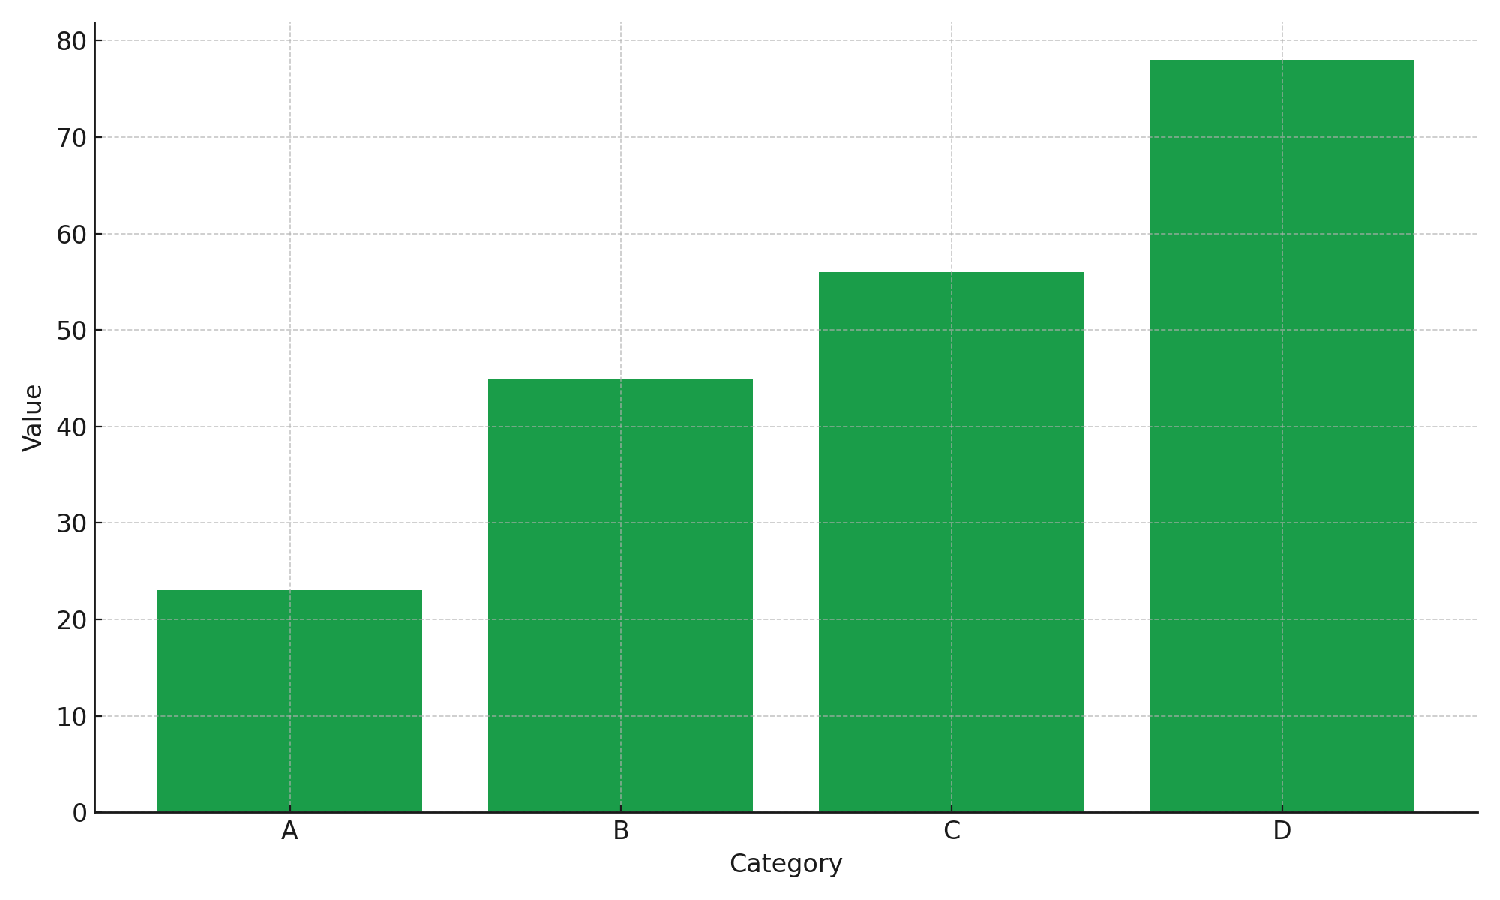
\includegraphics{./fig1.pdf}

\end{figure}%

\subsubsection{Python}\label{python}

Vi kan produsere figurer med kode. F.eks. kan man bruke Matplotlib til
dette:

\begin{Shaded}
\begin{Highlighting}[]
\InformationTok{\textasciigrave{}\textasciigrave{}\textasciigrave{}\{python\}}
\InformationTok{import pandas as pd}
\InformationTok{import matplotlib.pyplot as plt}

\InformationTok{\# Sample data}
\InformationTok{data = \{}
\InformationTok{    \textquotesingle{}Category\textquotesingle{}: [\textquotesingle{}A\textquotesingle{}, \textquotesingle{}B\textquotesingle{}, \textquotesingle{}C\textquotesingle{}, \textquotesingle{}D\textquotesingle{}],}
\InformationTok{    \textquotesingle{}Value\textquotesingle{}: [23, 45, 56, 78]}
\InformationTok{\}}

\InformationTok{\# Create DataFrame}
\InformationTok{df = pd.DataFrame(data)}

\InformationTok{\# Plotting the data}
\InformationTok{plt.figure(figsize=(10, 6))}
\InformationTok{plt.bar(df[\textquotesingle{}Category\textquotesingle{}], df[\textquotesingle{}Value\textquotesingle{}], color=\textquotesingle{}skyblue\textquotesingle{})}
\InformationTok{plt.xlabel(\textquotesingle{}Category\textquotesingle{})}
\InformationTok{plt.ylabel(\textquotesingle{}Value\textquotesingle{})}
\InformationTok{plt.title(\textquotesingle{}Sample Bar Plot\textquotesingle{})}
\InformationTok{plt.grid(axis=\textquotesingle{}y\textquotesingle{}, linestyle=\textquotesingle{}{-}{-}\textquotesingle{}, alpha=0.7)}
\InformationTok{plt.tight\_layout()}

\InformationTok{\# Show plot}
\InformationTok{plt.show()}
\InformationTok{\textasciigrave{}\textasciigrave{}\textasciigrave{}}
\end{Highlighting}
\end{Shaded}

Figure~\ref{fig-example1} viser at \ldots.

\begin{figure}

\caption{\label{fig-example1}Et eksempel på en graf produsert med
Matplotlib}

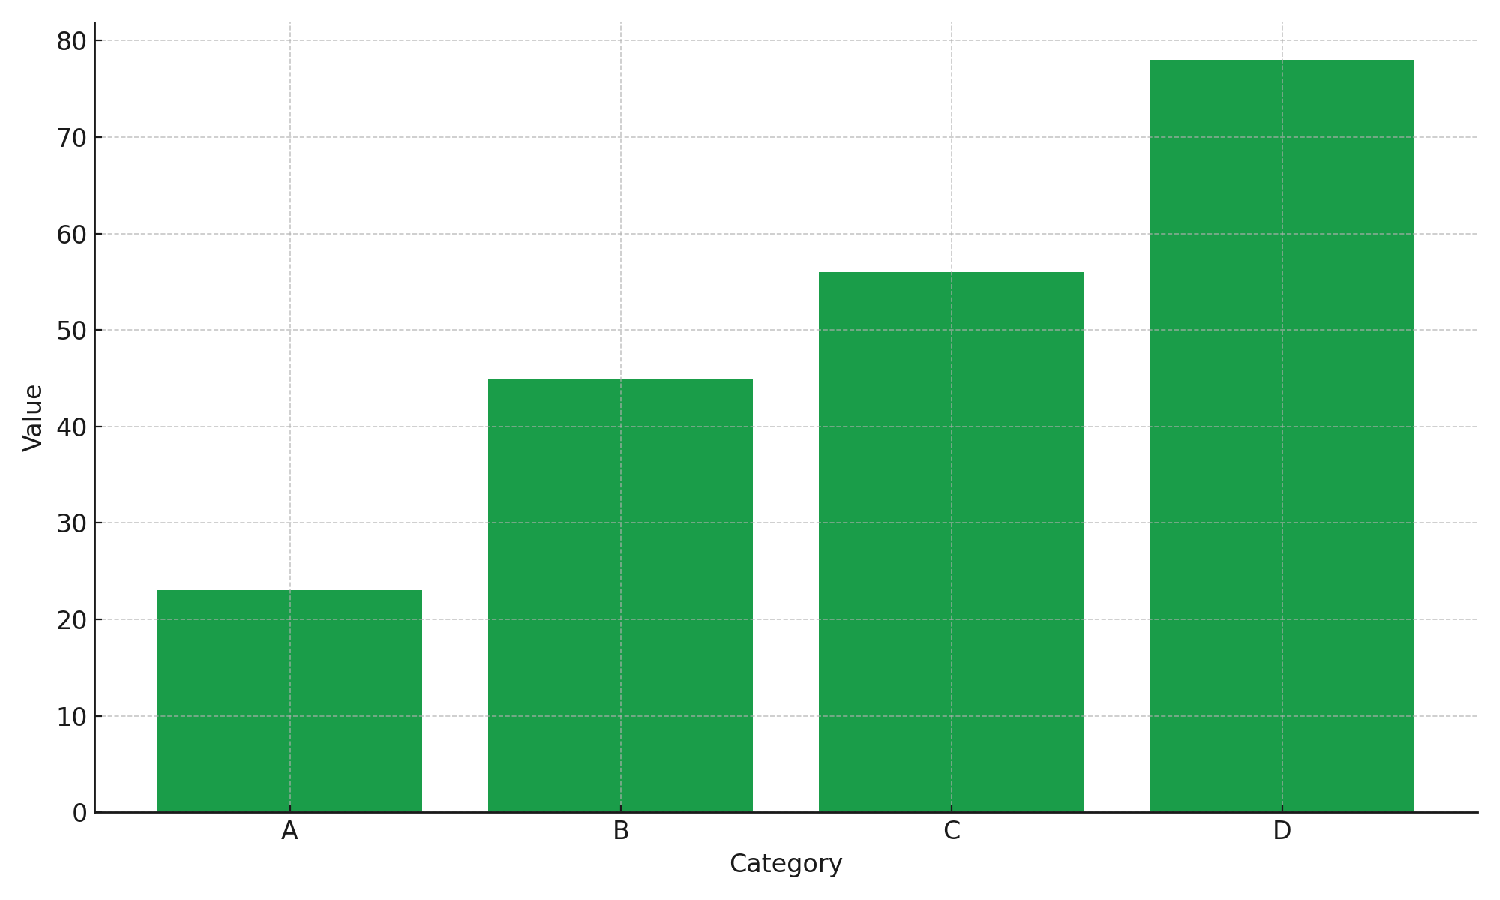
\includegraphics{./fig1.pdf}

\end{figure}%

\subsubsection{R}\label{r}

\begin{Shaded}
\begin{Highlighting}[]
\FunctionTok{library}\NormalTok{(ggplot2)}
\FunctionTok{library}\NormalTok{(showtext)}
\end{Highlighting}
\end{Shaded}

\begin{verbatim}
Loading required package: sysfonts
\end{verbatim}

\begin{verbatim}
Loading required package: showtextdb
\end{verbatim}

\begin{Shaded}
\begin{Highlighting}[]
\CommentTok{\# Example: Load the Roboto font}
\FunctionTok{font\_add\_google}\NormalTok{(}\StringTok{"Roboto"}\NormalTok{, }\StringTok{"roboto"}\NormalTok{)}
\FunctionTok{showtext\_auto}\NormalTok{()}

\NormalTok{data }\OtherTok{\textless{}{-}} \FunctionTok{data.frame}\NormalTok{(}
  \AttributeTok{Year =} \FunctionTok{rep}\NormalTok{(}\DecValTok{2000}\SpecialCharTok{:}\DecValTok{2020}\NormalTok{, }\DecValTok{2}\NormalTok{),}
  \AttributeTok{Value =} \FunctionTok{c}\NormalTok{(}\FunctionTok{rnorm}\NormalTok{(}\DecValTok{21}\NormalTok{, }\AttributeTok{mean =} \DecValTok{50}\NormalTok{, }\AttributeTok{sd =} \DecValTok{10}\NormalTok{), }\FunctionTok{rnorm}\NormalTok{(}\DecValTok{21}\NormalTok{, }\AttributeTok{mean =} \DecValTok{60}\NormalTok{, }\AttributeTok{sd =} \DecValTok{15}\NormalTok{)),}
  \AttributeTok{Group =} \FunctionTok{rep}\NormalTok{(}\FunctionTok{c}\NormalTok{(}\StringTok{"Group A"}\NormalTok{, }\StringTok{"Group B"}\NormalTok{), }\AttributeTok{each =} \DecValTok{21}\NormalTok{)}
\NormalTok{)}

\FunctionTok{ggplot}\NormalTok{(data, }\FunctionTok{aes}\NormalTok{(}\AttributeTok{x =}\NormalTok{ Year, }\AttributeTok{y =}\NormalTok{ Value, }\AttributeTok{color =}\NormalTok{ Group)) }\SpecialCharTok{+}
  \FunctionTok{geom\_line}\NormalTok{(}\AttributeTok{size =} \DecValTok{1}\NormalTok{) }\SpecialCharTok{+}
  \FunctionTok{geom\_point}\NormalTok{(}\AttributeTok{size =} \DecValTok{2}\NormalTok{) }\SpecialCharTok{+}
  \FunctionTok{scale\_color\_manual}\NormalTok{(}\AttributeTok{values =} \FunctionTok{c}\NormalTok{(}\StringTok{"\#1f78b4"}\NormalTok{, }\StringTok{"\#33a02c"}\NormalTok{)) }\SpecialCharTok{+} \CommentTok{\# Customize colors}
  \FunctionTok{theme\_minimal}\NormalTok{(}\AttributeTok{base\_family =} \StringTok{"roboto"}\NormalTok{) }\SpecialCharTok{+}
  \FunctionTok{theme}\NormalTok{(}
    \AttributeTok{text =} \FunctionTok{element\_text}\NormalTok{(}\AttributeTok{size =} \DecValTok{12}\NormalTok{),}
    \AttributeTok{axis.title =} \FunctionTok{element\_text}\NormalTok{(}\AttributeTok{size =} \DecValTok{14}\NormalTok{),}
    \AttributeTok{axis.text =} \FunctionTok{element\_text}\NormalTok{(}\AttributeTok{size =} \DecValTok{12}\NormalTok{),}
    \AttributeTok{legend.title =} \FunctionTok{element\_blank}\NormalTok{(),}
    \AttributeTok{legend.position =} \StringTok{"bottom"}\NormalTok{,}
    \AttributeTok{panel.grid.major =} \FunctionTok{element\_line}\NormalTok{(}\AttributeTok{color =} \StringTok{"grey80"}\NormalTok{),}
    \AttributeTok{panel.grid.minor =} \FunctionTok{element\_line}\NormalTok{(}\AttributeTok{color =} \StringTok{"grey90"}\NormalTok{),}
    \AttributeTok{plot.title =} \FunctionTok{element\_text}\NormalTok{(}\AttributeTok{size =} \DecValTok{16}\NormalTok{, }\AttributeTok{face =} \StringTok{"bold"}\NormalTok{),}
    \AttributeTok{plot.subtitle =} \FunctionTok{element\_text}\NormalTok{(}\AttributeTok{size =} \DecValTok{14}\NormalTok{)}
\NormalTok{  ) }\SpecialCharTok{+}
  \FunctionTok{labs}\NormalTok{(}
    \AttributeTok{title =} \StringTok{"Statistics Norway Styled Line Chart"}\NormalTok{,}
    \AttributeTok{subtitle =} \StringTok{"Sample Data from 2000 to 2020"}\NormalTok{,}
    \AttributeTok{x =} \StringTok{"Year"}\NormalTok{,}
    \AttributeTok{y =} \StringTok{"Value"}
\NormalTok{  )}
\end{Highlighting}
\end{Shaded}

\begin{verbatim}
Warning: Using `size` aesthetic for lines was deprecated in ggplot2 3.4.0.
i Please use `linewidth` instead.
\end{verbatim}

\includegraphics{template_files/figure-pdf/unnamed-chunk-3-1.pdf}

\subsection{Referanser}\label{referanser}

\subsection{Forklaringsbokser}\label{forklaringsbokser}

\begin{tcolorbox}[enhanced jigsaw, colbacktitle=quarto-callout-note-color!10!white, title=\textcolor{quarto-callout-note-color}{\faInfo}\hspace{0.5em}{Forklaringsboks}, colframe=quarto-callout-note-color-frame, opacityback=0, rightrule=.15mm, bottomrule=.15mm, arc=.35mm, coltitle=black, titlerule=0mm, bottomtitle=1mm, colback=white, left=2mm, leftrule=.75mm, toptitle=1mm, breakable, toprule=.15mm, opacitybacktitle=0.6]

Forklaringsboks er nyttig for oppsummere et fenomen.

\end{tcolorbox}

\section{Referanser}\label{referanser-1}

Vi kan referere til annen litteratur ved å legge inn informasjon i
\texttt{bibliography.bib}-fila og referere til de i teksten med en
\texttt{@} foran etterpå. F.eks. skrev \citet{bruer2022sykefravaer} og
\citet{von2021modeling} noen interessante artikler for noen år siden.

Strukturen til \texttt{bibliography.bib} er slik:

\begin{Shaded}
\begin{Highlighting}[]
\NormalTok{@article\{bruer2022sykefravaer,}
\NormalTok{  title=\{Sykefrav\{\textbackslash{}ae\}r og frafall fra arbeidsmarkedet. Betydningen av sammensetningen av sykemeldte\},}
\NormalTok{  author=\{Bruer{-}Skarsb\{\textbackslash{}o\}, \{\textbackslash{}O\}yvind and Vigtel, Trond Christian\},}
\NormalTok{  year=\{2022\},}
\NormalTok{  publisher=\{Statistisk sentralbyr\{\textbackslash{}aa\}\}}
\NormalTok{\}}

\NormalTok{@article\{von2021modeling,}
\NormalTok{  title=\{Modeling R\textbackslash{}\&D spillovers to productivity: The effects of tax credits\},}
\NormalTok{  author=\{von Brasch, Thomas and Cappelen, \{\textbackslash{}AA\}dne and Hungnes, H\{\textbackslash{}aa\}vard and Skjerpen, Terje\},}
\NormalTok{  journal=\{Economic Modelling\},}
\NormalTok{  volume=\{101\},}
\NormalTok{  pages=\{105545\},}
\NormalTok{  year=\{2021\},}
\NormalTok{  publisher=\{Elsevier\}}
\NormalTok{\}}
\end{Highlighting}
\end{Shaded}

\section{About Quarto Extensions formats And Quarto Journals
Article}\label{about-quarto-extensions-formats-and-quarto-journals-article}

First, please get familiar with the following resources:

\begin{itemize}
\tightlist
\item
  \href{https://quarto.org/docs/extensions/formats.html}{Creating
  Formats} in Quarto as part of the
  \href{https://quarto.org/docs/extensions/}{Extensions} mechanism.
\item
  \href{https://quarto.org/docs/journals/}{Journals Articles} for
  Quarto.
\end{itemize}

\section{Structure of this
repository}\label{structure-of-this-repository}

Everything for the extensions is in \texttt{\_extensions}. See Quarto
doc for details.

\begin{itemize}
\item
  In \texttt{partials}, you'll find the \texttt{.tex} partials that can
  be used and should be removed or tweaked,s
\item
  Your extension can make shortcodes and lua filters available. This
  document shows the effect of the one provided in the \texttt{aft}
  format.
\item
  \texttt{aft} format sets some defaults which are different from
  \texttt{pdf} or \texttt{html}, link setting links to URL in read
  inside PDF output.
\end{itemize}

Source repository for this template format can found on
\href{https://github.com/quarto-journals/article-format-template}{Github}

\subsection{\texorpdfstring{\texttt{\_extensions\textbackslash{}aft}}{\_extensions\textbackslash aft}}\label{extensionsaft}

In this folder you'll find everything that defines the extensions which
could be installed using \texttt{quarto\ install\ extension} or be part
of the template when using \texttt{quarto\ use\ template}

\begin{description}
\item[Format Metadata]
This is in \texttt{\_extension.yml} is where all the metadata about the
format are defined so that Quarto knows what to use. Adapt this file for
you own template.
\item[Partials]
In \texttt{partials}, there are the \texttt{.tex} files that will be
used as Pandoc's template. We provide here all the partials supported by
Quarto and custom one for this format. Quarto allows to provide partials
to ease the process of tweaking the default latex Pandoc's template and
keeping it up to date.\\
This template repo contains all the relevant partials that you can use
with Quarto \emph{as example}. We only tweaked \texttt{title.tex} to
show the usage of a custom partials called \texttt{\_custom.tex}.\\
\textbf{Only keep the partials that you need to tweak for the format you
are creating}

If you need to completely change the default template (i.g customizing
partials is not enough), then you need to provide your own template to
Pandoc based on
\href{https://github.com/quarto-dev/quarto-cli/blob/main/src/resources/formats/pdf/pandoc/template.tex}{\texttt{template.tex}}
and also using partials or not. This can be provided using the
\texttt{template} YAML key in \texttt{\_extension.yml} for Quarto to use
it.

This is considered advanced configuration as it will be harder to
maintain than only using partials but could be required for some
specific format. Be aware that this may lead to loose some Pandoc or
Quarto features tied to default \texttt{template.tex} content if you
remove some specific parts.
\item[Lua Filters]
Most of the time, custom formats will need Lua filters to provide
specific features like cross format supports or provides custom
shortcodes through the Quarto extension mechanism. Those filters will be
available to the user and could be used in the custom formats (according
to \texttt{\_extensions} metadata). We have provided two examples:

\begin{itemize}
\tightlist
\item
  \texttt{color-text.lua}, a Lua filter used to add color to inline text
  for PDF and HTML outputs using the same Markdown syntax
\item
  \texttt{shorcodes.lua}, a Lua filter which follow
  \href{https://quarto.org/docs/authoring/shortcodes.html\#custom-shortcodes}{Quarto
  custom shortcodes} guidelines to provide a
  \texttt{\{\{\textless{}\ LaTeX\ \ \textgreater{}\}\}} shortcode to
  nicely print LaTeX in PDF and HTML.
\end{itemize}

\textbf{Remove or replace with your own Lua filters}
\item[Format resources]
Resources required by the format needs to be available. We have provided
two examples:

\begin{itemize}
\tightlist
\item
  \texttt{te.bst} is a biblio style file for demo. It has been
  downloaded from
  https://www.economics.utoronto.ca/osborne/latex/TEBST.HTM
  (http://econtheory.org/technical/te.bst) - Licence
  \href{https://www.latex-project.org/lppl/}{LPPL}
\item
  \texttt{aft.cls} is a dummy class file for this example format. It is
  a copy of official \texttt{article.cls}, the one provided in LaTeX
  installation (i.e at \texttt{kpsewhich\ article.cls}) and renamed as
  example (Licence LaTeX Project Public License)
\item
  \texttt{custom.scss} is a style file to have a custom theme for our
  HTML format so that our Lua filter feature \texttt{color-tex.lua}
  works.
\end{itemize}

Those files are referenced within the \texttt{\_extension.yml} to be
used with our example format.

\textbf{Remove and replace with your own resources}
\item[\texttt{.quartoignore}]
Sometimes it is useful to have some files only needed for reference or
for development. They should be available in the source repository but
not downloaded to the user when \texttt{quarto\ use\ template} is used.

\textbf{Use \texttt{.quartoignore} to register such file and folder (one
file or folder per line)}
\item[\texttt{style-guide} folder]
For \texttt{quarto-journals} format, use \texttt{style-guide} folder to
include any documentation and resourced used for format creation, like a
journal style guide or original \texttt{.tex} template. This folder is
already added in \texttt{.quartoignore} in this example repo.

\textbf{Remove, rename or add to this folder}
\item[\texttt{template.qmd}]
This file is the template document that shows how to use the custom
format. It will be downloaded with other resource by
\texttt{quarto\ use\ template}, and even offered to be renamed if the
name \texttt{template.qmd} is used.

This file will usually use the custom format (here \texttt{aft-pdf} and
\texttt{aft-html}) and show how to use the template. When you'll copy
this template, you should be able to render this document to the demo
format.

\textbf{Adapt this file to provide a suitable template for your custom
format}
\item[Other files]
Other files are needed by the template and are usually user provided -
they are not part of the custom format.

Here \texttt{bibliography.bib} is here to demo the usage of the bst file
from the custom format.

\textbf{Remove this file and provide a suitable one for your template}
\end{description}

\newpage{}

\section{Checklist: Creating a custom
format}\label{checklist-creating-a-custom-format}

Here is the checklist to help you know what to modify:

\begin{itemize}
\tightlist
\item
  Read the resources mentioned at the top,
\item
  Use this template repo to create a new repository for your format
  (Click on ``Use this template'' to create new github repo)
\item
  Once you are acquainted with the content, remove the resources that
  are there only as example (see above)
\item
  Update README by replacing \texttt{aft} and
  \texttt{Article\ Format\ Template} mentions for your journal format
\item
  Keep only the template partials that you need to tweak, and add custom
  ones if needed
\item
  Add any Lua filters for shortcodes and other that would be useful to
  create the expected output format
\item
  Add any external resource your format will need, and that should be
  part of the extension format that will be downloaded,
\item
  Check \texttt{\_extension.yml} is updated correctly
\item
  Modify the skeleton \texttt{template.qmd} to your format and add any
  required resources to be downloaded to user.
\item
  Check \texttt{.quartoignore} is updated which everything that should
  not be downloaded.
\item
  Publish a demo of you format to github pages of the repo by using
  \texttt{quarto\ publish} command
\end{itemize}

\section{Demo of some features found in this demo journal
template}\label{demo-of-some-features-found-in-this-demo-journal-template}

\subsection{Shortcode demo}\label{sec-shortcode}

PDF are rendered using {\LaTeX} but it is best if one can use a Markdown
syntax for cross format support.

\texttt{} used in source is a shortcode syntax where the shortcode is
included in the extension folder \texttt{\_extensions}

\subsection{Code chunk}\label{sec-chunks}

This format hide chunks by default as option has been set in
\texttt{\_extension.yml} file.

\begin{Shaded}
\begin{Highlighting}[]
\CommentTok{\#| prompt: true}
\CommentTok{\# Loading some data but this chunk won\textquotesingle{}t be shown.}
\FunctionTok{data}\NormalTok{(}\StringTok{"quine"}\NormalTok{, }\AttributeTok{package =} \StringTok{"MASS"}\NormalTok{)}
\end{Highlighting}
\end{Shaded}

But you can set \texttt{echo} option to \texttt{true} locally in the
chunk

\begin{Shaded}
\begin{Highlighting}[]
\CommentTok{\#| echo: true}
\NormalTok{m\_pois }\OtherTok{\textless{}{-}} \FunctionTok{glm}\NormalTok{(Days }\SpecialCharTok{\textasciitilde{}}\NormalTok{ (Eth }\SpecialCharTok{+}\NormalTok{ Sex }\SpecialCharTok{+}\NormalTok{ Age }\SpecialCharTok{+}\NormalTok{ Lrn)}\SpecialCharTok{\^{}}\DecValTok{2}\NormalTok{, }\AttributeTok{data =}\NormalTok{ quine, }\AttributeTok{family =}\NormalTok{ poisson)}
\FunctionTok{summary}\NormalTok{(m\_pois)}
\end{Highlighting}
\end{Shaded}

\subsection{Using tables}\label{using-tables}

This is how you use tables and reference them:

\begin{longtable}[]{@{}
  >{\raggedright\arraybackslash}p{(\columnwidth - 4\tabcolsep) * \real{0.0661}}
  >{\raggedright\arraybackslash}p{(\columnwidth - 4\tabcolsep) * \real{0.5289}}
  >{\raggedright\arraybackslash}p{(\columnwidth - 4\tabcolsep) * \real{0.4050}}@{}}
\caption{Et eksempel på en tabell}\label{tbl-example}\tabularnewline
\toprule\noalign{}
\begin{minipage}[b]{\linewidth}\raggedright
Område
\end{minipage} & \begin{minipage}[b]{\linewidth}\raggedright
kolonne1
\end{minipage} & \begin{minipage}[b]{\linewidth}\raggedright
kolonne2
\end{minipage} \\
\midrule\noalign{}
\endfirsthead
\toprule\noalign{}
\begin{minipage}[b]{\linewidth}\raggedright
Område
\end{minipage} & \begin{minipage}[b]{\linewidth}\raggedright
kolonne1
\end{minipage} & \begin{minipage}[b]{\linewidth}\raggedright
kolonne2
\end{minipage} \\
\midrule\noalign{}
\endhead
\bottomrule\noalign{}
\endlastfoot
Datasett & navn & inneholder personopplysinger \\
Datasett & beskrivelse & Verdivurdering \\
Datasett & populasjon & bruksrestriksjoner (hvis relevant) \\
Datasett & versjon & bruksrestriksjonsdato (hvis relevant) \\
Datasett & versjonsbeskrivelse (ikke relevant for versjon 1) &
datatilstand \\
Datasett & geografisk dekningsområde & status \\
Datasett & & enhetstype \\
Datasett & & inneholder dato fom \\
Datasett & & inneholder dato tom \\
Datasett & & eier \\
Datasett & & versjon \\
Datasett & & datakilde \\
Datasett & & temporalitetstype \\
Datasett & & statistikkområde \\
Datasett & & nøkkelord \\
Variabel & navn & definisjonURI/definitionUri \\
\end{longtable}

Du kryssreferer til Table~\ref{tbl-example} på denne måten.

\subsection{Text color}\label{sec-summary}

Our format makes applying color on inline text possible using the
\texttt{{[}content{]}\{color=\textless{}name\textgreater{}\}} syntax.
Let's see an example.

Here we are using a special feature of our format which is the coloring
because \textcolor{mypink}{pink is a \textbf{nice} color}.

This is possible thanks to the Lua Filter included in the custom
extension format.

\subsection*{Using references}\label{using-references}
\addcontentsline{toc}{subsection}{Using references}

I did not read this book but it must be interesting.

Differences between \texttt{aft-html} and \texttt{aft-pdf}:

\begin{itemize}
\tightlist
\item
  For the HTML format, we are using Pandoc citeproc to include the
  bibliography. Here \texttt{reference-section-title} controls the title
  for the chapter that will be used.
\item
  For the PDF format, \texttt{natbib} is used by default and the
  bibliography is included with a title by the LaTeX template.
\end{itemize}

\section*{Appendix}\label{appendix}
\addcontentsline{toc}{section}{Appendix}

I am grateful for the insightful comments offered by the anonymous peer
reviewers at Books \& Texts. The generosity and expertise of one and all
have improved this study in innumerable ways and saved me from many
errors; those that inevitably remain are entirely my own responsibility.


% Ensure the references section starts on a new page
\newpage
\phantomsection
\renewcommand{\refname}{Referanser} % For articles
\renewcommand{\bibname}{Referanser} % For books and reports
\addcontentsline{toc}{section}{Referanser}
\bibliographystyle{te}
\bibliography{bibliography} % Replace 'references' with the name of your .bib file without the .bib extension
% Add lists of figures and tables at the end of the document


\newpage
\phantomsection % Correct the hyperlink location for TOC
\addcontentsline{toc}{section}{Figurregister} % Add entry to TOC with correct page number
\section*{Figurregister}
\renewcommand{\listfigurename}{} % Remove the "List of Figures" title
\vspace{-3em} % Adjust the vertical space as needed
\listoffigures
\thispagestyle{ssb-report-footer-header} % Ensure the page style is applied to the list of figures

\newpage
\phantomsection % Correct the hyperlink location for TOC
\addcontentsline{toc}{section}{Tabellregister} % Add entry to TOC with correct page number
\section*{Tabellregister}
\renewcommand{\listtablename}{} % Remove the "List of Tables" title
\vspace{-3em} % Adjust the vertical space as needed
\listoftables
\thispagestyle{ssb-report-footer-header} % Ensure the page style is applied to the list of tables

\end{document}
